\documentclass{article}
\usepackage[utf8]{inputenc}
\usepackage{amsmath}
\usepackage{graphicx}
\usepackage{subfig}
\usepackage{caption}
\usepackage{authblk}
\usepackage[a4paper,top=3cm,bottom=3cm,left=3cm,right=3cm]{geometry}
\usepackage{wrapfig}

\usepackage{ragged2e}
\usepackage{lipsum}
\usepackage{float}
\restylefloat{table}
\begin{document}

\title{Relazione sullo studio del moto oscillatorio smorzato di una molla}
\author{Daniele Hasou \\ mail: daniele.hasou@studenti.unimi.it \\ matricola 967555 \\ gruppo 3E \\ anno scolastico 2020-2021 }
\date{27 giugno 2021}
\maketitle

\newpage

\section{Introduzione}
In un ambiente ideale, una molla sospesa e libera di muoversi a cui sia attaccata una massa tende ad oscillare intorno alla posizione di equilibrio, seguendo l'equazione del moto:
\begin{equation}
    m\frac{d^2x}{dt^2}=-kx,
\end{equation}
dove $m$ rappresenta la massa appesa e $k$ la costante elastica della molla presa in esame. Sperimentalmente ci si rende però conto che il moto di tale molla viene smorzato da forze esterne, in particolare da forze di attrito, che seguono la forma
\begin{equation}
    (C_1+C_2|{\frac{dx}{dt}}|)\frac{dx}{dt}.
\end{equation}
Il valore delle costanti $C_1$ e $C_2$ non può essere stabilito a priori: oggetto di questo studio sarà analizzare il moto smorzato di una molla per stabilire il valore delle due costanti d'attrito. Per fare ciò, si ricostruirà il moto di diverse combinazioni massa-molla, analizzandone il comportamento. In particolare, verranno presi in considerazione solo i due casi $C_1=0$ e $C_2=0$, per i quali è possibile risolvere l'equazione differenziale del moto.
Per decidere quale tra i due casi sia compatibile con i risultati delle misurazioni, verranno utilizzati strumenti statistici ( il calcolo del $\chi^2$) che permettano un confronto tra curve sperimentali e curve teoriche.

\section{Trattazione teorica}
Si consideri una combinazione massa-molla (ovvero una molla a cui viene agganciata una massa) appesa ad un supporto che le consenta di oscillare lungo il suo asse verticale. Il moto di tale corpo, soggetto a forze d'attrito, è descritto dall'equazione differenziale:

\begin{equation}
    m\frac{d^2x}{dt^2}=-kx-(C_1+C_2|{\frac{dx}{dt}}|)\frac{dx}{dt},
\end{equation}
dove $m$ indica la massa appesa, $k$ la costante elastica della molla e la grandezza 
\begin{equation}
    -(C_1+C_2|{\frac{dx}{dt}}|)\frac{dx}{dt}
\end{equation}
il contributo della forza d'attrito.

Tale equazione può essere risolta in maniera analitica se $C_2=0$ e in maniera approssimata se $C_1=0$, ma è impossibile stabilire a priori quale tra i due casi si verifichi (o se nessuno dei due sia vero).\\



\subsection{Caso 1: $C_2=0$. Analisi teorica del moto}
Ponendo $C_2=0$ nella formula (3), si ottiene
\begin{equation}
     m\frac{d^2x}{dt^2}=-kx-C_1\frac{dx}{dt},
\end{equation}
equazione del moto armonico smorzato classico. Essa può essere ricondotta alla forma 
\begin{equation}
    \frac{d^2x}{dt^2}=-\omega_{0}^2x-2\gamma\frac{dx}{dt},
\end{equation}
con $\omega_{0}^2=\frac{k}{m}$ e $2\gamma=\frac{C_1}{m}$. L'equazione (6) è differenziale omogenea, e presenta due soluzioni in due principali casi differenti:
\begin{itemize}
    \item se $\omega_{0}^2\ll \gamma^2$, la molla segue un "$moto$ $sovrasmorzato$", secondo la legge oraria
    \begin{equation}
        x(t)=A_0e^{-\gamma t},
    \end{equation}
    in cui $A_0$ rappresenta l'allungamento massimo fornito inizialmente alla molla, mentre la componente $e^{-\gamma t}$ è un termine esponenziale decrescente con costante di tempo $\frac{1}{\gamma}$.
    \item se, al contrario, $\omega_{0}^2\gg \gamma^2$  la molla segue un "$moto$ $sottosmorzato$", descritto dalla legge oraria
    \begin{equation}
        x(t)=A_0e^{-\gamma t}cos(\sqrt{\omega_{0}^2-\gamma^2}t)
    \end{equation}
    che presenta, in aggiunta all'equazione (7), una componente che conferisce alla molla un moto ondulatorio con velocità angolare $\omega=\sqrt{\omega_{0}^2-\gamma^2}$.
    
\end{itemize}
(Il caso $\omega_{0}^2\sim \gamma^2$ si riconduce a una forma non oscillante dal comportamento simile al primo caso). Sperimentalmente, si nota con facilità che la molla, una volta messa in moto, compie numerose oscillazioni, e pertanto il suo moto sarà sottosmorzato e descritto dall'equazione (8). Dovrà essere  verificato che $\omega_{0}^2\gg \gamma^2$.


\subsection{Caso 2: $C_1=0$. Analisi teorica del moto}
Ponendo invece $C_1=0$ nella formula (3), si ottiene
\begin{equation}
    m\frac{d^2x}{dt^2}=-kx-C_2|{\frac{dx}{dt}}|\frac{dx}{dt}.
\end{equation}
Tale equazione può essere risolta mediante considerazioni sulla conservazione dell'energia.
In particolare, sapendo che l'equazione del moto smorzato tende ad assumere la forma
\begin{equation}
    x(t)=A(t)cos(\omega t),
\end{equation}
si può ricavare che la funzione $A(t)$ assuma la forma:
\begin{equation}
    A(t)=\frac{A_0}{1+A_0\alpha t}
\end{equation}
in cui la costante $\alpha$ è definita come
\begin{equation}
    \alpha=\frac{4}{3\pi}C_2\frac{\omega_0^3}{k}.
\end{equation}
L'unità di misura di $\alpha$ è $[\alpha]=\frac{1}{ms}$.\\
La risoluzione espressa dall'equazione (11) è in realtà valida fintanto che $C_2\ll \frac{m}{A}$, relazione che dovrà essere verificata.
\subsection{Differenza tra il caso $C_2=0$ e $C_1=0$ }
 \begin{figure}[h]
\centering
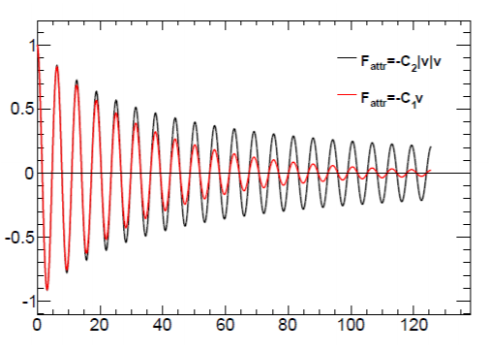
\includegraphics[width=0.5\textwidth]{c1 vs c2.png}
\caption{Ampiezza dell'oscillazione vs tempo. Si noti come l'ampiezza della curva rossa, che rappresenta il caso $C_2=0$, decresca molto più rapidamente rispetto al caso $C_1=0$}
\end {figure}
Per verificare se $C_1=0$ o $C_2=0$, risulta utile analizzare sperimentalmente se la curva seguita da una molla oscillante soggetta a forze d'attrito sia meglio descritta dall'equazione
\begin{equation}
    x(t)=A_0e^{-\gamma t}cos(\omega t)
\end{equation}
o dall'equazione
\begin{equation}
    x(t)=\frac{A_0}{1+A_0\alpha t}cos(\omega t).
\end{equation}
Le curve (13) e (14) sono comparate nella figura (1): come si osserva, la differenza nel comportamento delle due diventa più importante col passare del tempo. Risulta pertanto importante, al fine di ottenere risultati significativi, che vengano considerati tempi lunghi quando si ricerca di analizzare A(t).
    
\section{Metodi sperimentali e di analisi}
\subsection{Metodo di raccolta dati }

    
Per studiare l'andamento della funzione $A(t)$, si è deciso di analizzare i punti di massimo della funzione x(t). Per tali punti, infatti,  nell'equazione (10) la quantità $cos(wt)=1$ e dunque $x(t)=A(t)$: risulta agevole ricercare i valori che mappino la curva $A(t)$ studiando i massimi locali della curva $x(t)$, poichè questi coincidono.\\
E' stato pertanto progettato un esperimento che permettesse di ottenere i valori dei massimi di ciascuna oscillazione. Diverse combinazioni di masse e molle sono state analizzate e i risultati sono stati comparati. 

   
\subsection{Apparato sperimentale, strumenti ed errori strumentali}
Per la realizzazione di questa esperienza sono state usate:

\begin{itemize}
    \item Due molle, dotate di due anelli ad entrambe le estremità. Di queste molle sono note le costanti elastiche (con relativo errore) e le masse (con relativo errore). I valori sono riportati nella tabella sottostante.\\ 
            \begin{table*}[h]
  \begin{center}
    \begin{tabular}{c|c|c}
     molla  &  costante elastica $k$ [$\frac{N}{kg}$] & massa [g] \\ \hline
             1  & 3,12\pm0,03 & 15,2\pm0,1 \\
            2  & 24,4\pm0,1 &29,4\pm0,1 \\
    \end{tabular}
  \end{center}
  \caption{costante elastica e massa delle due molle utilizzate per l'esperimento}
\end{table*}
            
            
    
   

   
 
    \item Alcuni pesi cilindrici di massa nota (con errore $\sigma_{massa}=0,01g$).
    \item Un supporto per i pesi, di massa $28,20\pm0,01g$, dotato di un gancio che permette di ancorarlo ad un anello di una molla. Esso presenta una base circolare ampia.
    \item Un sensore a onde sonore, in grado di registrare e trasmettere la distanza che lo separa da un corpo, fornendo le informazion con la precisione di $0,0001m$.
    \item Il software PASCO Capstone, che, ricevendo dati dal sensore, è in grado di rappresentarli su un grafico e studiarne l'andamento.
    \item Tre aste rigide ed alcuni morsetti che le tengano in posizione.
    
\end{itemize}


Affinché la raccolta dati fosse efficiente, era necessario che la molla fosse libera di muoversi solo nella direzione verticale, e che a modificare il suo moto fossero unicamente le forze di attrito con l'aria. Per garantire ciò, è stata realizzata una struttura rigida utilizzando le tre aste, ponendone due in verticale (fissate saldamente al tavolo) e una in orizzontale (ancorata alle altre due mediante i morsetti). Grazie all'anello presente all'estremità della molla, questa è stata agganciata all'asta orizzontale, in modo che fosse libera di oscillare ma non potesse scorrere. La rigidità della struttura ha permesso che il moto della molla non si trasmettesse ad altri elementi del sistema.

All'anello inferiore della molla è stato agganciato il supporto per i pesi, in cui è stata inserita una combinazione di pesi accuratamente scelta dallo sperimentatore. 
Per registrare la posizione della 
\begin{wrapfigure}{r}{6cm}
    \caption{rappresentazione schematizzata dell'apparato sperimentale. }\label{wrap-figura:1}
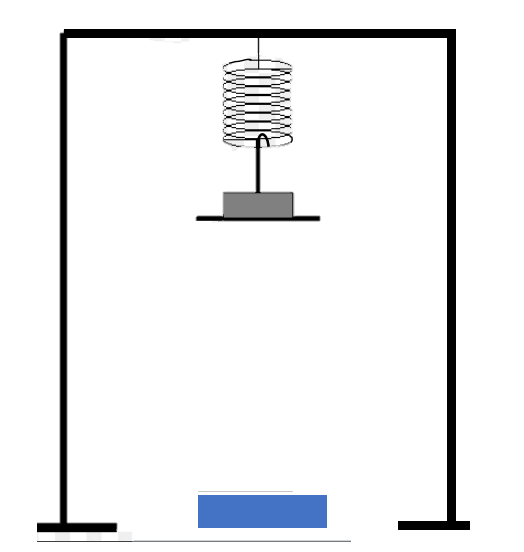
\includegraphics[width=6cm]{setup definitivo (2).png}
\end{wrapfigure}
molla in funzione del tempo, il sensore a onde sonore (il corpo blu nella figura 2) è stato posto esattamente sotto al supporto dei pesi, che, con la sua ampia base circolare, aiutava affinché venissero registrate misure valide. \\

Grazie al software PASCO Capstone, in un primo momento è stata misurata la "distanza a riposo" (ovvero la distanza tra il supporto e il sensore quando la molla è in condizione di equilibrio) di ciascuna combinazione massa-molla con il rispettivo errore. Messo in moto il sistema (semplicemente spingendo verso il basso il supporto), il sensore, con una frequenza fornita dallo sperimentatore (scelta a 100Hz), ha rilevato la distanza dalla base del supporto e l'informazione è stata rielaborata dal software Capstone, che ha ricreato per ogni combinazione massa-molla una approssimazione della curva del moto. A partire da tali dati, è stato possibile ricavare le distanze massime del supporto dal sensore in funzione del tempo (sottraendo alle distanze massime di ogni combinazione massa-molla la distanza di equilibrio specifica). 


    

\subsection{Metodo di analisi dei dati}
Per studiare in maniera efficiente il moto smorzato della molla e analizzare i due casi prima mostrati, occorre  costruire le curve che seguano l'andamento espresso nella componente A(t) delle formule (13) e (14) che meglio si adattino ai dati sperimentali. Per comodità, sono state ricercate delle trasformazioni che, mantenendo l'integrità dell'esperimento, permettessero  di linearizzare le curve, facilitando la ricerca dei parametri col rispettivo errore. Nella seconda metà dell'analisi dei dati, sono state confrontate la retta ottenuta dalla regressione lineare con la curva ottenuta attraverso le trasformazioni dei dati. Lo studio sulla compatibilità delle due curve ha fornito le informazioni necessarie per stabilire il comportamento del sistema.
\subsubsection{Propagazione dell'errore} 
Prevedendo di dover attuare trasformazioni sui dati per poter procedere alla linearizzazione, è necessario attuare di volta in volta la propagazione dell'errore per ogni valore. Data una funzione $G(x, y, z)$, si ha:
\begin{equation}
    \sigma_G=\sqrt{\left [\frac{\partial G}{\partial x}\right]^2\sigma_x^2+\left[\frac{\partial G}{\partial y}\right]^2\sigma_y^2+\left[\frac{\partial G}{\partial z}\right]^2\sigma_z^2}
\end{equation}\\
In particolare, se la funzione è a solo un'incognita, si ha
\begin{equation}
    \sigma_G=\sqrt{\left [\frac{\partial G}{\partial x}\right]^2\sigma_x^2}=|\frac{\partial G}{\partial x}|\sigma_x
\end{equation}

\subsubsection{Caso $C_2=0$: trasformazioni dei dati e strumenti per la linearizzazione}
\'E già stato mostrato come, per questa situazione, avendo posto $cos(\omega t)=1$ si abbia 
\begin{equation*}
    A(t)=A_0e^{-\gamma t},
\end{equation*}
 
con $A_0$ ampiezza iniziale del moto.
Sapendo che il moto seguito dalla molla è periodico, i massimi vengono raggiunti in ogni istante di tempo del tipo $t=t_0+nT$, con $T$ periodo dell'oscillazione e $t_0$ istante in cui si registra il primo massimo. Ponendo $t_0=0$  tutti gli altri massimi avverranno a $nT$. Si può dunque scrivere:
\begin{equation}
    \frac{x(T)}{x(nT)}=\frac{A_0e^{-\gamma T}}{A_0e^{-\gamma nT}}=e^{(n-1)\gamma T}.
\end{equation}
Ponendo il logaritmo ad ambo i membri, si ottiene
\begin{equation}
    ln( \frac{x(T)}{x(nT)})=(n-1)\gamma T
\end{equation}
riconducibile facilmente alla forma $y=Bx$ con $y=ln( \frac{x(T)}{x(nT)})$ e $x=(n-1)$.
Per ottenere il valore del coefficiente angolare $B$, è necessario, dopo aver attuato le necessarie trasformazioni sui dati, usare la formula per la regressione lineare per la retta passante per l'origine, ovvero
\begin{equation}
    B=\frac{\sum_{i}x_iy_i}{\sum_{i}x_i^2}
\end{equation}
con 
\begin{equation}
    \sigma_B^2=\frac{\sigma_y^2}{\sum_{i}x_i^2}.
\end{equation}
La grandezza $\sigma_y$ deve essere ricavata con la propagazione dell'errore a partire da ogni valore $x(nT)$. In particolare,
\begin{equation}
    \sigma_y=\sigma_A \sqrt{\frac{1}{x(T)^2}+\frac{1}{x(nT)^2}}
\end{equation}
dove $\sigma_A$ rappresenta l'incertezza sulle ampiezze dell'oscillazione.
Si noti come i vari $\sigma_y$ differiscano tra loro; per il calcolo di $\sigma_B$ verrà scelto il valore $\sigma_y$ più grande.

Il valore del periodo (col rispettivo errore) viene calcolato computando la media e la deviazione standard della media degli intervalli di tempo che trascorrono tra un punto di massimo e il successivo, come mostrato nelle formule:
\begin{equation}
     \Bar{T}=\frac{\sum_{i=1}^{n} T_i}{n},
\end{equation}
\begin{equation}
    \sigma_{\Bar{T}}=\sqrt{\frac{\sum_{i=1}^{n} (T_i-\Bar{T})^2}{N(N-1)}}
\end{equation}
\subsubsection{Caso $C_1=0$: trasformazioni dei dati e strumenti per la linearizzazione}
E' stato mostrato come in questo caso la funzione $A(t)$ segua un andamento del tipo
\begin{equation}
    A(t)=\frac{A_0}{1+A_0\alpha t}
\end{equation}
in cui $A_0$ rappresenta l'ampiezza dell'oscillazione iniziale e $\alpha$ è definita
\begin{equation}
    \alpha=\frac{4C_2\omega_0^3}{3\pi k}.
\end{equation}
In particolare, sapendo che $x(t)=A(t)$, è possibile riscrivere l'equazione (15) come 
\begin{equation}
    \frac{1}{x(nT)}=\frac{1}{A_0}+\alpha nT,
\end{equation}
riconducibile alla forma $y=A+Bx$ imponendo $y=\frac{1}{x(nT)}$ e $x=nT$. In questo caso, contrariamente al precedente, per effettuare la regressione lineare è necessario considerare diverso da $0$ il termine noto. Si avrà dunque:
\begin{align*}
    A=\frac{\sum_{i}x_i^2\sum_{i}y_i-\sum_{i}x_i\sum_{i}x_iy_i}{\Delta}; \ \ \ & \sigma_A=\sqrt{\frac{\sum_{i}x_i^2}{\Delta}}\sigma_y\\
    B=\frac{N\sum_{i}x_iy_i-\sum_{i}x_i\sum_{i}y_i}{\Delta}; \ \ \ & \sigma_B=\sqrt{\frac{N}{\Delta}}\sigma_y \\
\end{align*}
con 
\begin{equation*}
    \Delta=N\sum_{i}^{N}x_i^2-(\sum_{i}^{N}x_i)^2
\end{equation*}
Il periodo T e il suo errore saranno calcolati come mostrato nel paragrafo precedente, mentre l'errore $\sigma_y$ è dato da
\begin{equation}
   \sigma_y=\frac{\sigma_A}{x(nT)^2}
\end{equation}
\subsubsection{Metodo per il confronto tra curve }
Per decidere se uno dei due casi proposti sia sufficientemente adatto a rappresentare la situazione empirica, si  è scelto di effettuare un test del chi quadro. In particolare, poiché deve essere analizzata la compatibilità con rette, per calcolare il $\chi^2$ è possibile usare la formula:
\begin{equation}
    \chi^2=\sum_{j}\left[\frac{y_{j}-Bx_j-A}{\sigma_{y_j}}\right]^2,
\end{equation}
dove $B$ e $A$ ricavati dalla linearizzazione (ovviamente nel caso $C_2=0$ si avrà il termine noto $A=0$).
Confrontando i valori del test del $\chi^2$ ottenuti con i gradi di libertà (GDL) di ogni test, si potrà discutere la compatibilità tra la curva teorica e la curva ottenuta.

\section{Risultati sperimentali}
\subsection{Scelta della combinazione massa-molla}
Per studiare maglio gli effetti dell'attrito è necessario ricostruire la curva $A(t)$ per intervalli di tempo sufficientemente lunghi, come spiegato in precedenza. Per ottenere una ricostruzione della curva $A(t)$ più fitta, si è scelto di analizzare combinazioni massa-molla caratterizzate da una frequenza sufficientemente alta (arbitrariamente maggiore di 1 Hz), che permettono di ottenere una quantità di dati significativa in un intervallo di tempo definito. \\
Per scegliere le combinazioni massa-molla con questa proprietà, sono stati ricostruiti grazie all'uso del sensori i moti di diverse combinazioni, e sono state registrate le relative frequenze. Si è notato che aumentando la massa del sistema diminuiva la frequenza di oscillazione: sono dunque state scelte combinazioni che garantissero sia una frequenza maggiore di 1 Hz, sia risultati più chiari. Riducendo la massa appesa, infatti, ci si è resi conto empiricamente che si manifestavano con maggiore frequenza i problemi proposti nel paragrafo 4.6"Errori sperimentali".  \\

\\
\\

Per la molla 1 sono state scelte due diverse combinazioni massa-molla, per analizzare come mutasse il comportamento del sistema al variare della massa. I valori delle combinazioni scelte sono segnati nella tabella sottostante (inclusa la "distanza di equilibrio"). \\

\begin{table*}[h]
  \begin{center}
    \begin{tabular}{c|c|c|c|c}
     molla  & k [N/kg]  & massa appesa [g] & frequenza [Hz] & $l_{eq}$ [m] \\ \hline
    1 & 3,12 \pm 0,02 & 47,71 \pm 0,02 & 1,22 \pm $10^{-4}$ & 0,2840\pm0,0001\\
    1 & 3,12 \pm 0,02 & 28,20 \pm 0,01 & 1,53 \pm $10^{-4}$ & 0,3468\pm0,0001\\
    2 & 24,4 \pm 0,1 & 207,68 \pm 0,03 & 1,67 \pm $10^{-4}$ & 0,2022\pm0,0001\\
    \end{tabular}
  \end{center}
  \caption{frequenze di oscillazione e distanza di equilibrio dal sensore per le diverse combinazioni massa-molla usate nell'esperimento}
\end{table*}

\subsection{Esperienza di raccolta dei massimi}
Usando il procedimento spiegato nel paragrafo 3.2, sono stati ricostruiti tramite il sensore e il software online PASCO Capstone i moto oscillatori di ogni combinazione e sono stati individuate tutte le distanze massime ("$x_{max}")$ dal sensore. Tali valori sono stati considerati con un'incertezza pari a $\sigma_{dist.max}=0,0002 m$, in quanto si è assunto che i valori di massimo individuati dal sensore non corrispondessero ai massimi effettivi (poiché il campionamento della posizione della molla non era continuo). 
\\ Per risalire ai valori delle ampiezze delle oscillazioni, si ha semplicemente calcolato per ogni valore
\begin{equation}
    A(t)= x_{max}(t)-l_{eq},
\end{equation}
ricordando di effettuare la propagazione degli errori, per la quale si ottiene
\begin{equation}
    \sigma_A=\sqrt{\sigma_{dist.max}^2+\sigma_{eq}^2}=0,00022m.
\end{equation}
I valori così ottenuti, che mappano $A(t)$, sono stati registrati nei grafici sottostanti. \\

\begin{figure}[h]
\centering
\subfloat[][\emph{andamento di $A(t)$ per la combinazione molla 1-massa 47,71g}]
{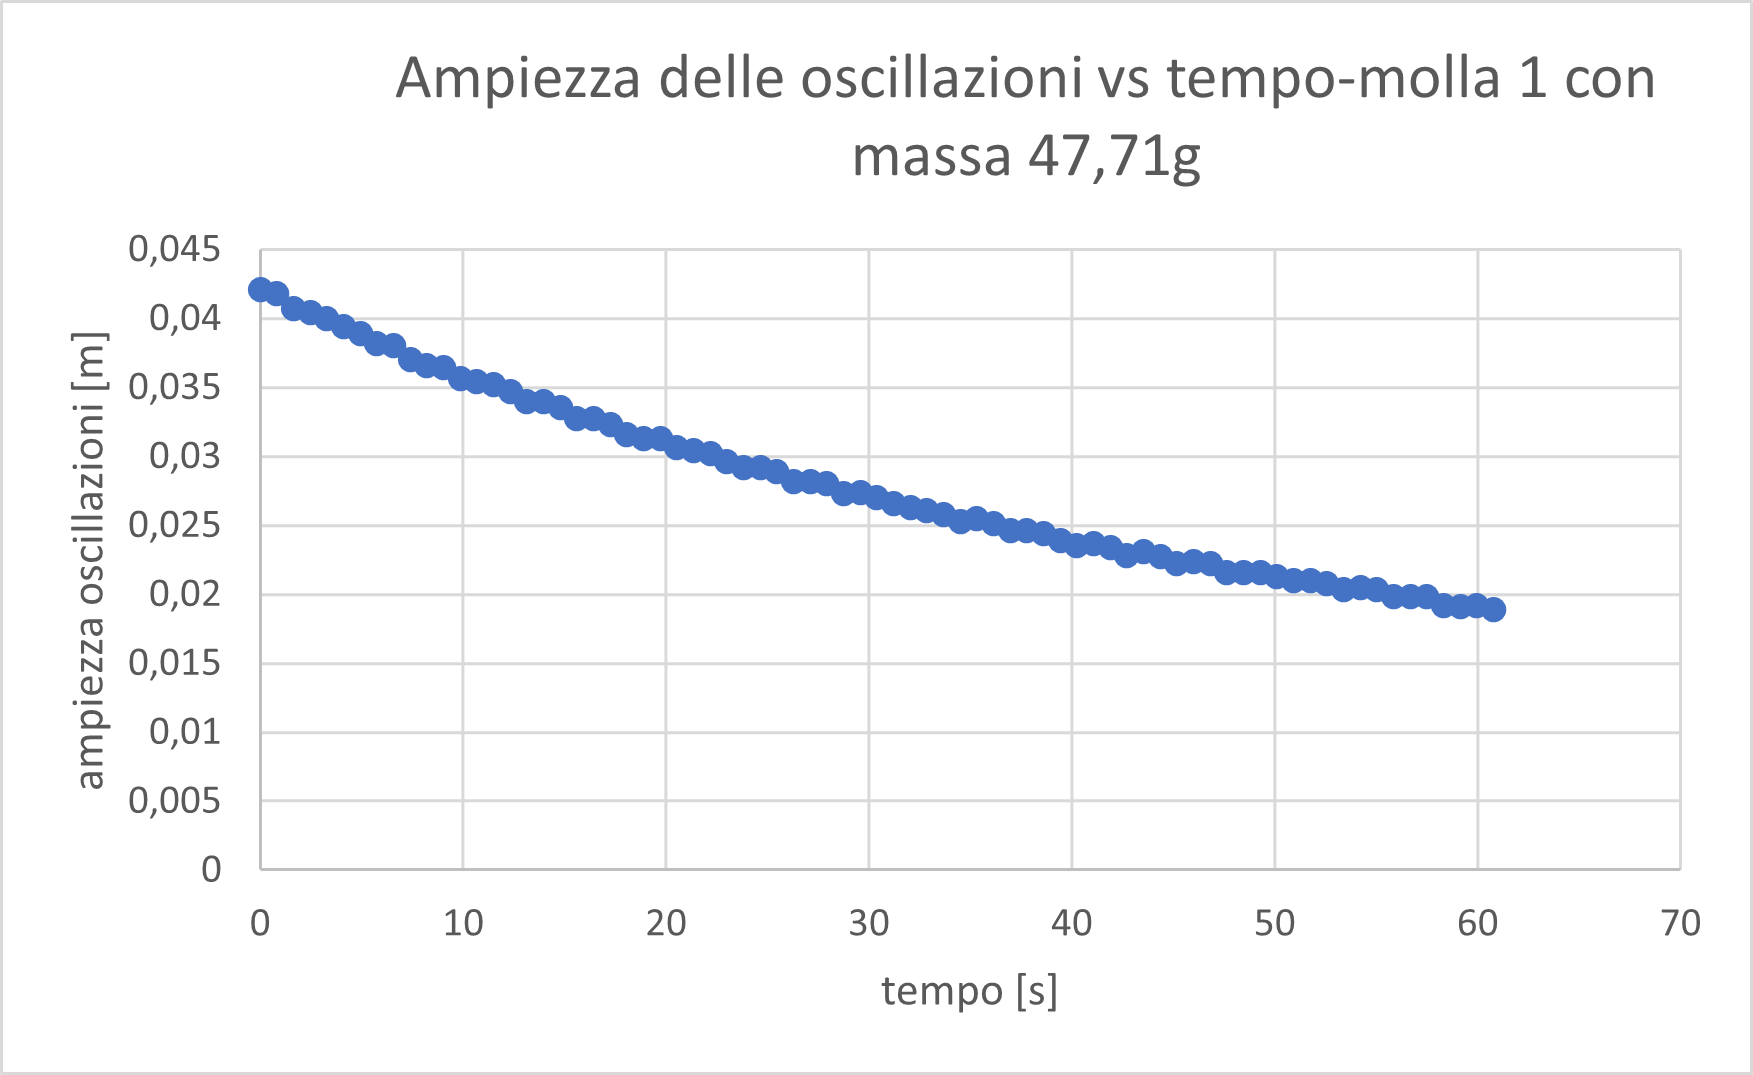
\includegraphics[width=.45\textwidth]{grafico molla 1 47 grammi a(t) definitivo.png}} \quad
\subfloat[][\emph{andamento di $A(t)$ per la combinazione molla 1-massa 28.20g}]
{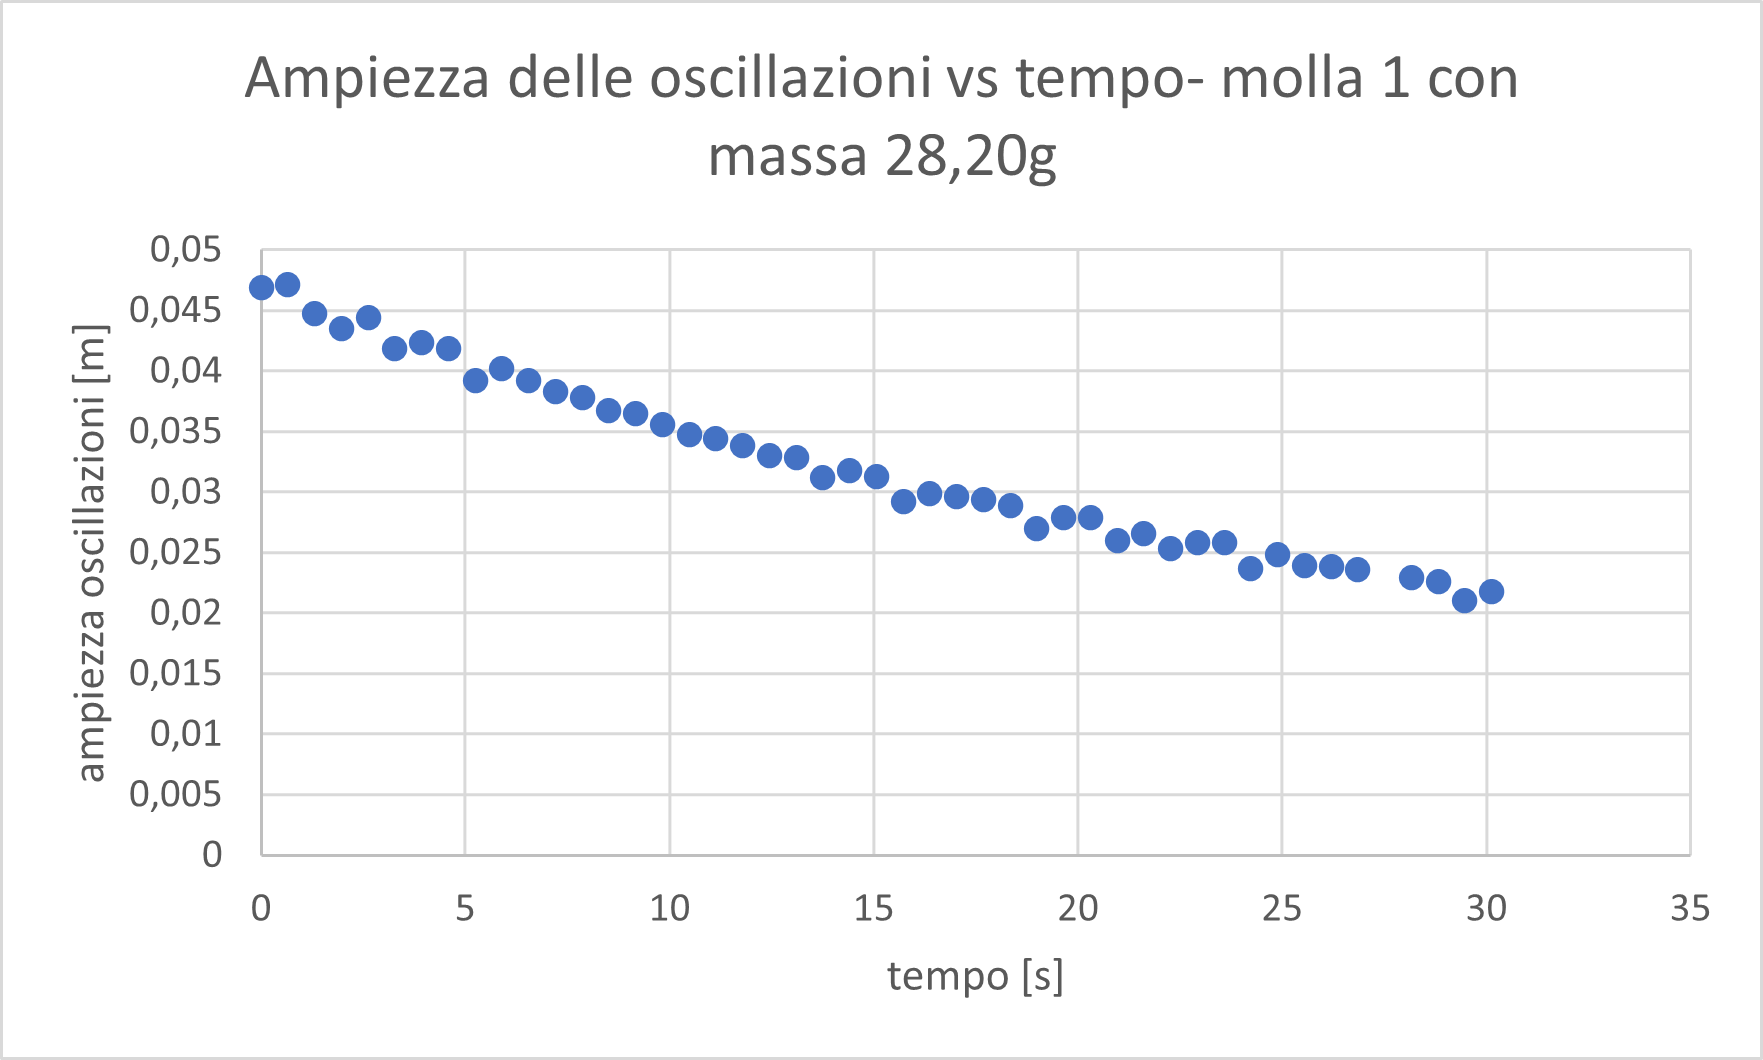
\includegraphics[width=.45\textwidth]{grafico molla 1 28 grammi a(t).png}} \\
\subfloat[][\emph{andamento di $A(t)$ per la combinazione molla 2-massa 207,68g}]
{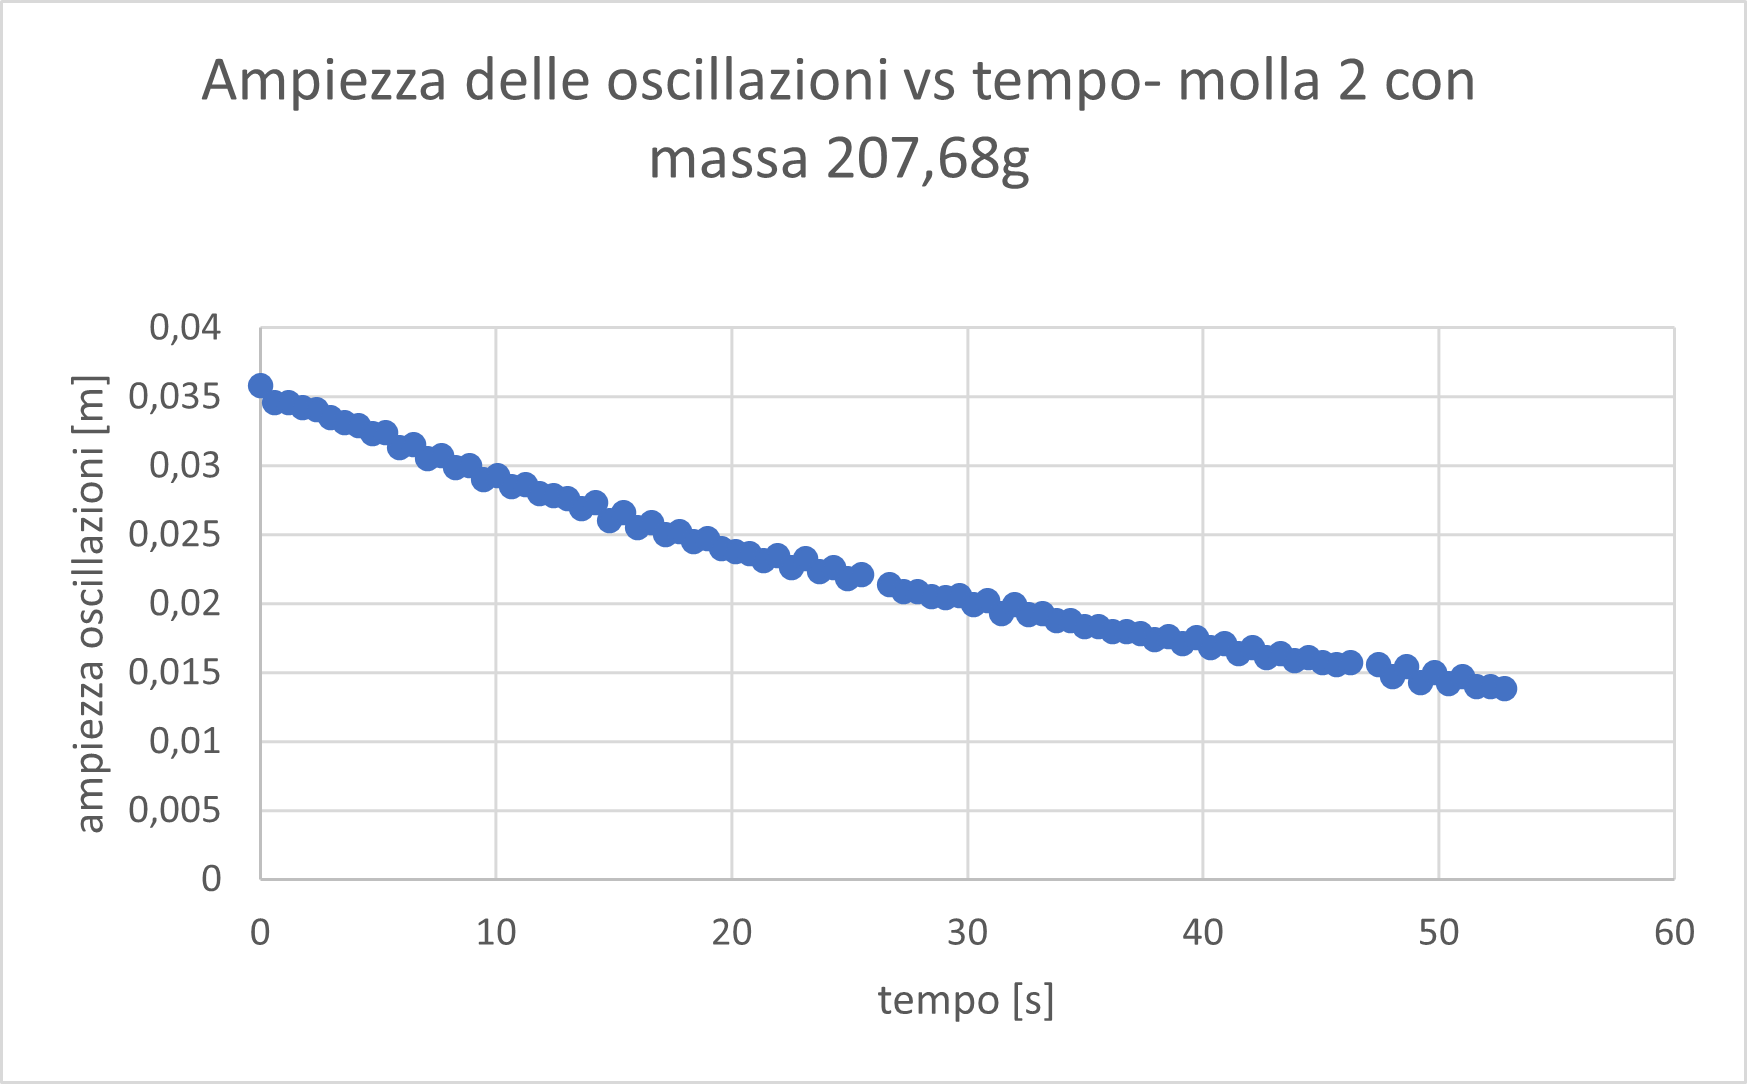
\includegraphics[width=.45\textwidth]{grafico molla 2 a(t).png}} \quad

\caption{I grafici mostrano l'andamento della funzione $A(t)$ per le diverse combinazioni massa-molla.}
\label{fig:subfig}
\end{figure}

Usando questi valori, è stato possibile attuare le regressioni lineari spiegate in precedenza.
\subsection{Analisi dei dati}
\subsubsection{Caso 1: $C_2=0$. Analisi dei dati sperimentali}
Ai dati ottenuti sono state applicate le trasformazioni necessarie per la regressione lineare definiti nel paragrafo 3.3.2-"caso $C_2=0$: trasformazione dei dati e strumenti per la linearizzazione".\\
Sull'asse orizzontale sono state poste dunque le grandezze $(n-1)$, mentre sull'asse verticale le grandezze $ln(\frac{x(T)}{x(nT)})$. \\ I dati della regressione sono mostrati nella tabella sotto (3):\\ \\
\begin{table*}[h]
  \begin{center}
    \begin{tabular}{c|c|c}
     molla & massa appesa [g] & B della retta [$s^{-1}$]  \\ \hline
     1 & 47,71\pm0,02 & 0,0114\pm$3\times10^{-5}$  \\
     1 & 28,20\pm0,01 & 0,0175\pm$5\times10^{-5}$  
\\
     2 & 207,68 \pm 0,03 & 0,0110 \pm $3\times10^{-5}$  \\
    \end{tabular}
  \end{center}
  \caption{la tabella riporta i coefficienti angolari delle rette che meglio si adattano ai dati sperimentali trasformati mediante i metodi spiegati nel paragrafo 3.3.2}
\end{table*}

\\ \\
Per il calcolo delle costanti $\gamma$ sono stati calcolati i periodi di ogni oscillazione con relativa incertezza (ricordando che $B=\gamma t)$, usando le formule (22) e (23). I valori ottenuti sono stati registrati nella tabella sottostante (4).\\
\begin{table*}[h]
  \begin{center}
    \begin{tabular}{c|c|c|c}
     molla & massa appesa [g] & periodo oscillazione [s] & $\gamma$ [$s^{-1}$] \\ \hline
    1 & 47,71\pm0,02 & 0,8215\pm0,001 & 0,0139\pm$4\times10^{-5}$\\
    1 & 28,20\pm0,01 & 0,655\pm0,001 & 0,0267\pm$1\times10^{-4}$ \\
    2 & 207,68\pm0,03 & 0,593\pm0,001 & 0,0186\pm$6\times10^{-5}$\\
    \end{tabular}
  \end{center}
  \caption{la tabella riporta i valori dei periodi di oscillazione e della costante $\gamma$ per le diverse combinazioni}
\end{table*}\\
Considerando che $\omega=2\pi f$, usando i dati contenuti nella tabella (2) si vede che può essere confermata la relazione $\gamma^2\ll\omega^2$, come richiesto nel paragrafo 2.1.

\subsubsection{Caso 2: $C_1=0$. Analisi dei dati sperimentali}
Come per il caso precedente, sono state attuate le trasformazioni spiegate nel paragrafo 3.3.3:"caso $C_1=0$: trasformazione dei dati e strumenti per la linearizzazione", ponendo sull'asse orizzontale $(nT)$ (utilizzando i periodi calcolati in precedenza) e su quello verticale la grandezza $\frac{1}{x(nT)}$. \\
In questo caso, avendo su entrambi gli assi quantità che presentano un errore, è necessario verificare che $\sigma_y$ sia più significativo che $\sigma_x$. I valori sono riportati nella tabella (5). In particolare, sono riportati i massimi di tali valori. \\ 
\begin{table*}[h]
  \begin{center}
    \begin{tabular}{c|c|c|c}
     molla & massa appesa [g] & errore x (percentuale) & errore y (percentuale) \\ \hline
     1 & 47,71\pm0,02 & 0,001 & 0,012 \\
    1 & 28,20\pm0,01 & 0,001 & 0,010 \\
    2 & 207,68\pm0,03 & 0,001& 0,016 \\
    \end{tabular}
  \end{center}
  \caption{la tabella mostra i valori degli errori percentuali sulle grandezze poste sull'asse orizzontale e verticale. Si dimostra che è lecito effettuare una regressione lineare non pesata, dal momento che l'errore sull'asse verticale è molto più significativo.}
\end{table*}\\
Come si può vedere, la condizione è verificata: si può dunque applicare linearizzazione non pesata, ottenendo i valori mostrati nella tabella (6).
\begin{table*}[h]
  \begin{center}
    \begin{tabular}{c|c|c|c}
      molla & massa appesa [g] & B=\alpha \  [$(m\times s)^{-1}$] & A [$m^{-1}$]\\ \hline
    1 & 47,71\pm0,02 & 0,478\pm0,004 & 23,00\pm0,14 \\
    1 & 28,20\pm0,01 & 0,828\pm0,009 &  20,33\pm0,15\\
    2 & 207,68\pm0,03 & 0,820\pm0,008 &  26,04\pm0,23\\
    \end{tabular}
    \caption{la tabella mostra i valori del coefficiente angolare e del termine noto ottenuti tramite la regressione lineare nel caso $C_1=0$. Si ricorda che $\alpha$ corrisponde al coefficiente angolare della retta}
  \end{center}
  
\end{table*}\\
Per verificare la condizione $C_2\ll \frac{m}{A}$, basta considerare gli ordini di grandezza delle quantità interessate: per la molla 1, $C_2$ è dell'ordine di $10^{-4}$, $m$ dell'ordine di $10^{-2}$ e $A$ dell'ordine di $10^{-2}$.

\newpage
\subsection{Confronto tramite il calcolo del $\chi^2$}
Una volta realizzata la linearizzazione, è possibile confrontare le curve ottenute mediante le trasformazioni con le rette trovate, usando il metodo del $\chi^2$ (formula 28). Nelle tabelle sono forniti i valori del $\chi^2$ per ogni combinazione massa-molla, inclusi i gradi di libertà di ogni per ogni caso e la probabilità di compatibilità, prima per il caso $C_2=0$ poi per il caso $C_1=0$. \\

\begin{table*}[h]
  \begin{center}
    \begin{tabular}{c|c|c|c|c}
      molla  &  massa & \chi^2 & GDL & probabilità\\ \hline
     1 & 47,71\pm0,02 & 421 & 74 & $ \ll0,01$\\
    1 & 28,20\pm0,01 & 284 & 45 &  $ \ll0,01$\\
    2 & 207,68\pm0,03 & 340 & 87 & $ \ll0,01$\\
    \end{tabular}
  \end{center}
  \caption{in tabella sono fornite le informazioni su $\chi^2$, gradi di libertà e relativa probabilità di compatibilità per ogni combinazione massa-molla, relative al caso $C_2=0$}
\end{table*}\\
\begin{table*}[h]
  \begin{center}
    \begin{tabular}{c|c|c|c|c}
       molla  &  massa & \chi^2 & GDL & probabilità\\ \hline
     1 & 47,71\pm0,02 & 236 & 73 & $ \ll0,01$ \\
    1 & 28,20\pm0,01 & 596 & 44 & $ \ll0,01$\\
    2 & 207,68\pm0,03 & 302 & 86 & $ \ll0,01$\\
    \end{tabular}
  \end{center}
  \caption{in tabella sono fornite le informazioni su $\chi^2$, gradi di libertà e relativa probabilità di compatibilità per ogni combinazione massa-molla, relative al caso $C_1=0$}
\end{table*}
  
 
 

\subsection{Analisi dei risultati}
Il confronto col $\chi^2$ mostra chiaramente come nessuna delle curve ottenute sperimentalmente possa essere ritenuta statisticamente compatibile. Questo porta ad affermare che né il modello $C_2=0$ né quello $C_1=0$ descrivono accuratamente il moto smorzato della molla.\\
\'E comunque importante far notare che durante il processo di raccolta dei dati, diversi problemi sono sorti, descritti nella sezione successiva. Questi problemi, che si è cercato di risolvere o di rimuovere il più possibile, potrebbero aver sensibilmente aumentato l'incertezza sulle misure raccolte.\\ 
I risultati ottenuti portano ad affermare che a regolare il moto smorzato per le tre combinazioni non sia in particolare una sola delle due costanti, ma una combinazione di entrambe.\\
Degno di nota il comportamento delle costanti $\alpha$ e $\gamma$ nelle due combinazioni della molla 1. I valori mostrano  che per la combinazione più leggera le ampiezze decrescono più rapidamente che per la combinazione più pesante. 
\subsection{Errori sperimentali}
Durante la raccolta dati si sono presentate diverse situazioni che avrebbero potuto portare a errori sperimentali considerevoli. Si riportano l'errore, un modo per accorgersene e una soluzione:
\begin{itemize}
    \item Il grafico che viene registrato presenta minimi costanti nel tempo, mentre i massimi seguono un andamento decrescente: questo è dovuto ad uno scorretto posizionamento della molla rispetto al sensore. Il sensore, infatti, non è in grado di registrare con precisione le distanze dei corpi posti troppo vicini ad esso. Per risolvere questo problema, basta posizionare l'asta orizzontale più in alto o il sensore su un ripiano più basso. 
    Questo non costituisce un problema eccessivo a meno che la molla non compia il suo intero moto di oscillazione a distanze scorrette.
    \item Il grafico presenta per lo più un andamento decrescente, ma alcuni punti si trovano particolarmente disallineati rispetto agli altri: è dovuto a problemi nel moto di oscillazione o allo scorretto posizionamento del sensore rispetto alla base del supporto. \'E possibile che una parte molto piccola dell'oscillazione verticale si trasformi in oscillazione orizzontale (introducendo un moto tipo pendolo) senza che si noti ad occhio. Questo è difficile da eliminare, ma per migliorare la presa dati si può agganciare la molla ad un filo a sua volta annodato all'asta verticale: allungando la lunghezza verticale del sistema massa-molla, diminuiscono gli effetti di tale problema. 
    \begin{figure}[h]
\centering
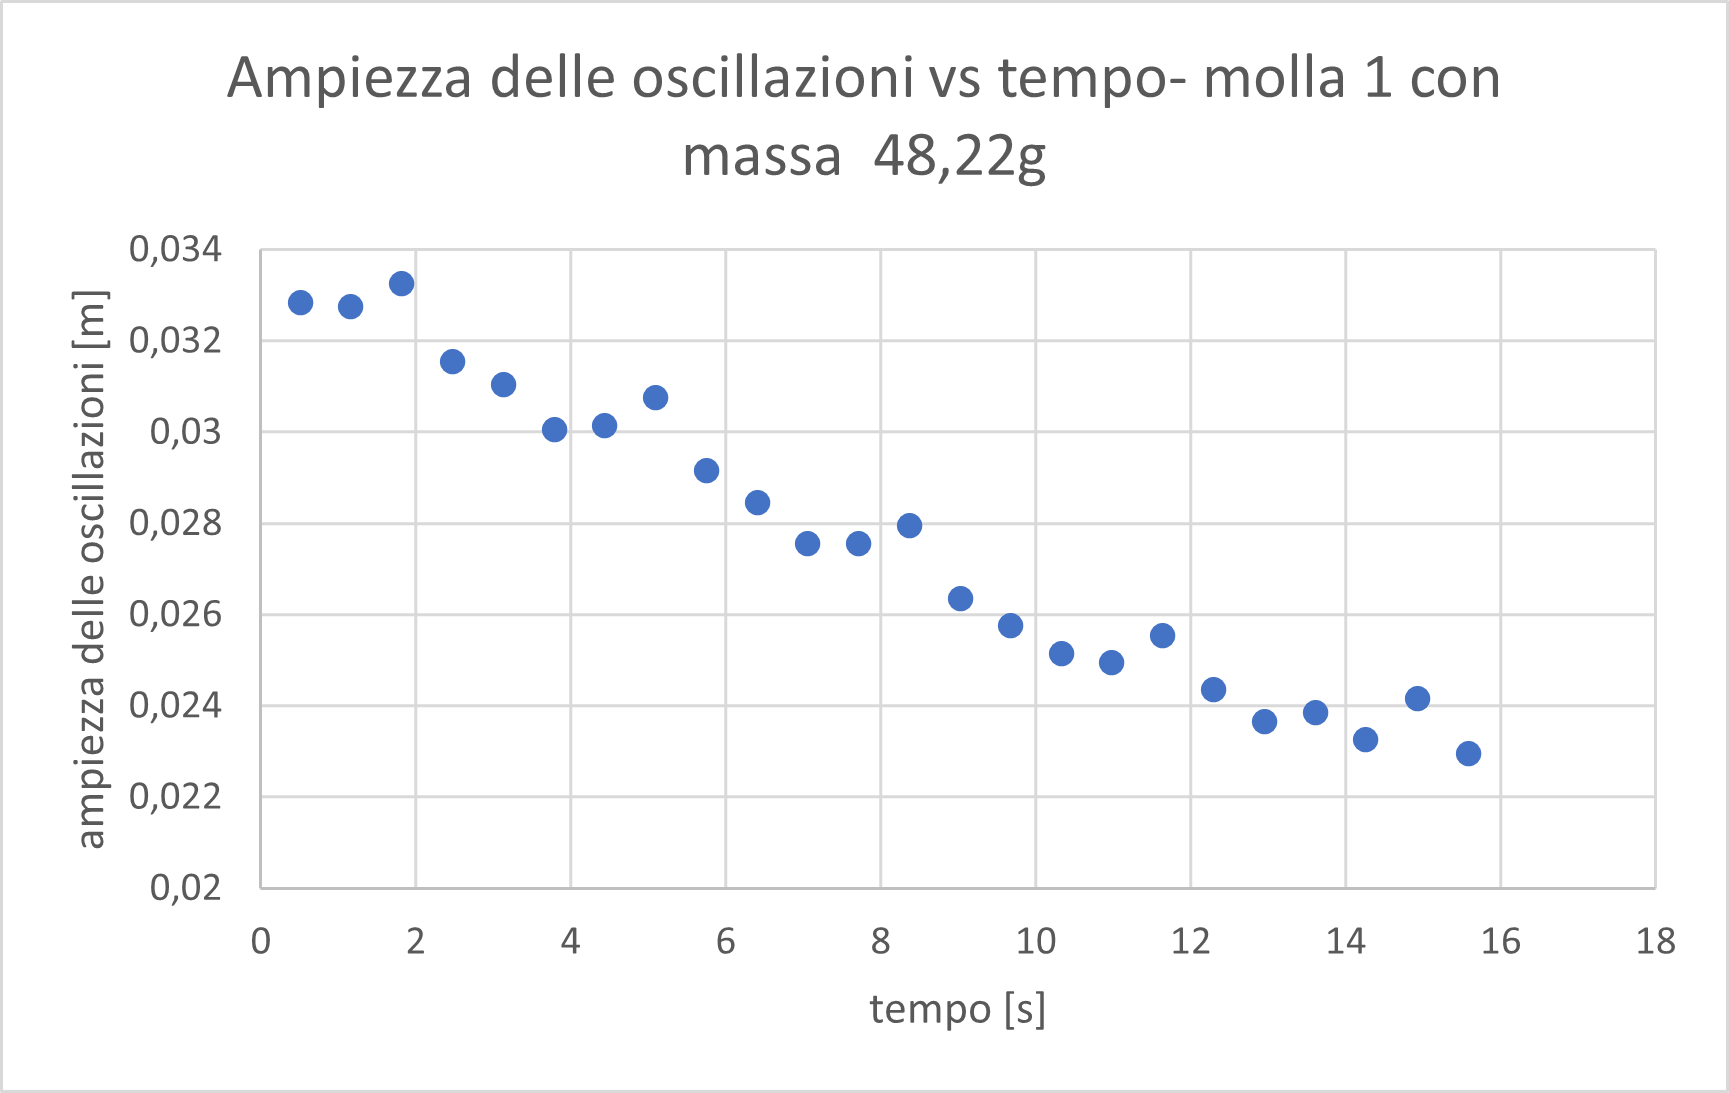
\includegraphics[width=0.5\textwidth]{grafico sbagliato.png}
\caption{Ampiezza dell'oscillazione vs tempo per la combinazione molla 1-massa 48,22g. Si noti l'andamento regolare ma visibilmente incoerente rispetto alla curva attesa.}
\end {figure}
    \item La molla comincia visibilmente a oscillare non solo in orizzontale ma anche in verticale: tale problema potrebbe essere dovuto a una scorretta spinta iniziale. Bisogna assicurarsi che la spinta si perfettamente allineata con la verticale della molla. Come si nota, alcune combinazioni massa-molla sono più suscettibili a questo tipo di problemi (in particolare, combinazioni con masse leggere), e ampiezze iniziali troppo grandi possono contribuire a questo problema. 
    
\end{itemize}



\section{Conclusione}
Obiettivo di questa esperienza è stato quello di studiare il comportamento di una molla libera di contrarsi e dilatarsi ma soggetta a forze d'attrito. In particolare, in relazione all'equazione 
\begin{equation}
    m\frac{d^2x}{dt^2}=-kx-(C_1+C_2|{\frac{dx}{dt}}|)\frac{dx}{dt},
\end{equation} 
presentata inizialmente, si è cercato di analizzare le due costanti $C_1$ e $C_2$, concentrandosi sui casi $C_1=0$ e $C_2=0$. 

Nessuna delle tre combinazioni massa-molla selezionate ha compiuto un moto statisticamente comparabile ai due casi sopracitati, come mostrato dal test del $\chi^2$ che è stato effettuato. I risultati di tale test individuano probabilità minori dell'1\% di compatibilità tra le curve teoriche e le curve ottenute a partire dai dati sperimentali: da ciò si evince che l'equazione del moto seguito dal sistema sia caratterizzato da una combinazione di $C_1$ e $C_2$.



\end{document}
